\chapter{مفاهیم اولیه}
در این فصل به معرفی مقدمات و مفاهیم مورد نیاز در این پایان‌نامه می‌پردازیم. 
\section{مقدمه}
در این بخش به تاریخچه هوش مصنوعی، دستاورد های اولیه، چالش ها، دلایل رکود هوش مصنوعی و پایان عصر تاریک هوش مصنوعی صحبت میکنیم 

% update the abstract


\chapter{مفاهیم اولیه}

در این فصل به معرفی مقدمات و مفاهیم مورد نیاز در این پایان‌نامه می‌پردازیم.

\section{مقدمه}

در این بخش به تاریخچه هوش مصنوعی، دستاوردهای اولیه، چالش‌ها، دلایل رکود هوش مصنوعی و پایان عصر تاریک هوش مصنوعی صحبت می‌کنیم.

\subsection{آغاز هوش مصنوعی و هدف اصلی}

هوش مصنوعی به عنوان شاخه‌ای از علوم کامپیوتر، در دهه ۱۹۵۰ با هدف ساخت سیستم‌ها و ماشین‌هایی که توانایی تقلید از هوش انسانی را دارند، آغاز شد. نخستین بار، مکارتی در سال ۱۹۵۶ این اصطلاح را به کار گرفت \cite{mccarthy1956proposal} و هوش مصنوعی به عنوان علمی که در آن به مطالعه الگوریتم‌هایی برای تقلید رفتار انسانی می‌پردازد، شناخته شد. اهداف اولیه هوش مصنوعی شامل توانایی درک زبان، یادگیری، حل مسئله و تولید موجودات هوشمند بود. در این دوران پروژه‌های تحقیقاتی زیادی به امید دستیابی به هوش مصنوعی عمومی 
(\lr{AGI, Artificial General Intelligence})
شروع به کار کردند \cite{crevier1993ai,nilsson2010quest}.

\subsection{دورهٔ طلایی و پیشرفت‌های اولیه}

در دههٔ ۵۰ و ۶۰ میلادی، هوش مصنوعی به عنوان یکی از پرچمداران پژوهش‌های نوین شناخته می‌شد. الگوریتم‌های اولیه با تکیه بر روش‌های منطقی و ریاضیاتی برای حل مسئله و بازی‌های ساده توسعه یافتند؛ مانند انواع الگوریتم‌های جستجوی درختی که در این دوره به وجود آمدند و زمینه‌ساز اولین دستاوردهای هوش مصنوعی در بازی‌های تخته‌ای همچون شطرنج شدند \cite{newell1959report}. در این دوران، پیشرفت‌های بیشتری در پردازش زبان طبیعی (\lr{NLP}) و سیستم‌های خبره (\lr{Expert Systems}) نیز صورت گرفت که این امید را در دانشمندان و محققان تقویت کرد که دستیابی به هوش مصنوعی عمومی به‌زودی ممکن خواهد بود \cite{feigenbaum1983handbook}.

\subsection{انتظارات بیش از حد و ظهور عصر تاریک}

با وجود پیشرفت‌های هوش مصنوعی، محدودیت‌های تکنولوژی (مثل عدم وجود \lr{GPU}های پرقدرت در آن زمان) و همچنین کمبود داده‌های کافی برای آموزش مدل‌های پیچیده‌تر، باعث شد که بسیاری از پروژه‌های تحقیقاتی نتوانند به نتایج پیش‌بینی‌شده دست یابند. در نتیجه، هوش مصنوعی در دههٔ ۷۰ به مرحله‌ای از رکود وارد شد که به آن عصر تاریک هوش مصنوعی یا \lr{AI Winter} می‌گویند \cite{lighthill1973artificial,crevier1993ai}. در این دوران، بسیاری از پروژه‌ها تعطیل و سرمایه‌گذاری‌ها قطع شدند و دولت‌ها و سازمان‌های سرمایه‌گذار به دلیل عدم دستیابی به نتایج مطلوب از ادامهٔ سرمایه‌گذاری منصرف شدند.

\subsection{عوامل اصلی عصر تاریک هوش مصنوعی}

\begin{itemize}
	\item \textbf{محدودیت‌های سخت‌افزاری:}  
	در آن زمان، سیستم‌های اولیهٔ هوش مصنوعی به محاسبات سنگینی نیاز داشتند که با توان پردازشی محدود آن دوره همخوانی نداشت \cite{nilsson2010quest}.
	
	\item \textbf{کمبود داده‌ها:}  
	در آن زمان، دسترسی به داده‌های کافی برای آموزش مدل‌های پیچیده ممکن نبود و الگوریتم‌های موجود به داده‌های بیشتری نیاز داشتند تا بتوانند به‌درستی آموزش ببینند و عملکرد مطلوبی داشته باشند \cite{crevier1993ai}.
	
	\item \textbf{روش‌های محدود یادگیری:}  
	الگوریتم‌های اولیه به شدت به برنامه‌ریزی انسانی وابسته بودند و در بسیاری از موارد، مدل‌ها قادر به تعمیم به مسائل جدید نبودند و نمی‌توانستند تعمیم‌پذیری خیلی بالایی داشته باشند \cite{russell2016artificial}.
\end{itemize}

\subsection{پایان عصر تاریک و بازگشت هوش مصنوعی}

پس از چندین سال رکود و عدم سرمایه‌گذاری در حوزهٔ هوش مصنوعی، سرانجام در دههٔ ۱۹۸۰ و ۱۹۹۰ عصر تاریک هوش مصنوعی با تحولات تکنولوژی و از همه مهم‌تر ظهور سیستم‌های خبره (\lr{Expert Systems}) به پایان رسید \cite{feigenbaum1983handbook}. سیستم‌های خبره به عنوان یکی از اولین تلاش‌های موفق برای کاربردهای صنعتی در هوش مصنوعی به‌وجود آمدند. بر خلاف الگوریتم‌های اولیه، این سیستم‌ها از پایگاه بزرگ قواعد و قوانین (\lr{Rule-Based Systems}) استفاده می‌کردند. در سیستم‌های خبره، به جای تلاش برای شبیه‌سازی کلی هوش مصنوعی، بر حل مسائل تخصصی برای صنایع و سازمان‌ها تمرکز می‌شد. برای مثال، سیستم‌های خبره در پزشکی برای تشخیص بیماری‌ها و پیشنهاد درمان، در صنعت برای مدیریت و پیش‌بینی خرابی ماشین‌آلات، و در امور مالی برای تحلیل و ارزیابی ریسک کاربرد داشتند \cite{mccorduck2004machines}.

هرچند این سیستم‌ها نمی‌توانستند درک عمیق و هوشمندی عمومی را ایجاد کنند، اما برای رفع نیازهای پیچیده مناسب بودند. همزمان با موفقیت این سیستم‌ها، بهبودهای زیادی در سخت‌افزارها و کاهش هزینه‌های پردازش به وجود آمد. در دهه‌های ۱۹۸۰ و ۱۹۹۰، کامپیوترها به تدریج قوی‌تر و مقرون به صرفه‌تر شدند و امکان پردازش داده‌های بیشتر و اجرای الگوریتم‌های پیچیده‌تر فراهم شد. این افزایش توان محاسباتی، نیاز به پردازش داده‌های بزرگ و پیچیده را برآورده کرد و در نتیجه دسترسی به داده‌ها و انجام محاسبات سنگین برای توسعهٔ الگوریتم‌های جدید تسهیل شد. از سوی دیگر، پیشرفت‌های انجام‌شده در ذخیره‌سازی داده و رشد اینترنت باعث دسترسی گسترده‌تر به داده‌ها و منابع اطلاعاتی گردید \cite{nilsson2010quest}.

به این ترتیب، مجموعه‌ای از عوامل، شامل ظهور سیستم‌های خبره، افزایش قدرت پردازش و دسترسی به داده‌های بیشتر، منجر به بازگشت هوش مصنوعی شد. این دوره نه تنها پایان عصر تاریک هوش مصنوعی بود، بلکه راه را برای الگوریتم‌های یادگیری ماشین و توسعهٔ شبکه‌های عصبی هموار کرد \cite{russell2016artificial}.


\section{انواع مدل یادگیری ماشین و شبکه‌های عصبی}\label{sec:ml-types}
یادگیری ماشین و شبکه‌های عصبی در سال‌های اخیر مورد توجه بسیاری قرار گرفته‌اند و در حوزه‌های متنوعی از جمله پردازش تصویر، پردازش زبان طبیعی و داده‌کاوی استفاده می‌شوند
\cite{bishop2006pattern,mitchell1997machine,murphy2012machine}.

\subsection{یادگیری ماشین: مروری کلی}
یادگیری ماشین (\lr{Machine Learning}) شاخه‌ای از هوش مصنوعی است که به مدل‌های محاسباتی این امکان را می‌دهد الگوها را از داده‌ها به شکل خودکار یاد بگیرند و بتوانند تصمیم‌گیری کنند
\cite{goodfellow2016deep,mitchell1997machine}.
در واقع، هدف یادگیری ماشین این است که مدل‌ها بتوانند از داده‌ها الگوها و روابط پنهان را استخراج کنند و به نتایج و تصمیم‌های قابل اعتماد دست یابند.

\subsection{تقسیم‌بندی‌های اصلی در یادگیری ماشین}
به طور کلی، یادگیری ماشین به سه دستهٔ اصلی تقسیم می‌شود:
\begin{itemize}
	\item یادگیری با نظارت (\lr{Supervised Learning})
	\item یادگیری بدون نظارت (\lr{Unsupervised Learning})
	\item یادگیری تقویتی (\lr{Reinforcement Learning})
\end{itemize}
این طبقه‌بندی در بسیاری از کتاب‌ها و مراجع مهم یادگیری ماشین مطرح شده است
\cite{bishop2006pattern,murphy2012machine}.

\subsection{یادگیری نظارت‌شده (\lr{Supervised Learning})}
یادگیری نظارت‌شده یکی از رایج‌ترین روش‌ها در یادگیری ماشین شناخته می‌شود که در آن از مجموعه داده‌های برچسب‌گذاری‌شده برای آموزش مدل استفاده می‌کنیم
\cite{james2013introduction}. هدف این الگوریتم تشخیص الگوها در میان داده‌های ورودی است تا بتواند روی داده‌های جدید پیش‌بینی یا طبقه‌بندی انجام دهد. این نوع شامل دو دسته الگوریتمِ \lr{Regression} و \lr{Classification} می‌شود.

\subsubsection{طبقه‌بندی (\lr{Classification})}
طبقه‌بندی یکی از مهم‌ترین و اصلی‌ترین وظایف در یادگیری نظارت‌شده است که هدف آن تخصیص هر داده به یک لیبل مشخص است
\cite{bishop2006pattern}.
در این روش، مدل با داده‌های برچسب‌دار (Label) آموزش می‌بیند و یاد می‌گیرد که داده‌های جدید را بر اساس الگوها و ویژگی‌هایی که در داده‌های آموزشی دیده است، به دسته مناسب اختصاص دهد. از کاربردهای طبقه‌بندی می‌توان به تشخیص اسپم (\lr{Spam Detection})، تشخیص بیماری (مثلاً آیا یک فرد مبتلا به بیماری هست یا نه) و تشخیص چهره اشاره کرد
\cite{murphy2012machine}.

\subsubsection{رگرسیون (\lr{Regression})}
رگرسیون یکی از مهم‌ترین وظایف یادگیری ماشین است و هدف آن پیش‌بینی مقادیر پیوسته است
\cite{montgomery2021introduction}. بر خلاف طبقه‌بندی که خروجی آن یک دسته‌بندی مجزا است، در رگرسیون خروجی یک مقدار پیوسته خواهد بود و مدل می‌آموزد روابط بین متغیرهای مستقل و متغیر هدف را شناسایی کند. از کاربردهای رگرسیون می‌توان به پیش‌بینی قیمت مسکن یا پیش‌بینی آب‌وهوا اشاره کرد.

\subsection{یادگیری تقویتی (\lr{Reinforcement Learning})}
یادگیری تقویتی، نوعی یادگیری بر پایهٔ پاداش و تنبیه است که در آن مدل با محیط تعامل می‌کند و بر اساس پاداش یا تنبیه یاد می‌گیرد
\cite{sutton2018reinforcement}.
برخلاف یادگیری نظارت‌شده و بدون نظارت، یادگیری تقویتی به مدل این امکان را می‌دهد تا از طریق آزمون و خطا بهترین راهکارها را برای انجام یک عمل یاد بگیرد. در این روش، مدل به جای برچسب، از یک تابع پاداش استفاده می‌کند که مشخص می‌کند چه اقداماتی باعث نتیجهٔ بهینه می‌شود. از کاربردهای یادگیری تقویتی می‌توان به بازی‌ها (\lr{Games})، کنترل رباتیک (\lr{Robotic Control}) و سیستم‌های توصیه‌گر (\lr{Recommender Systems}) اشاره کرد.


\subsection{معرفی چند مدل از الگوریتم یادگیری کلاسیک}

\subsubsection{نزدیک‌ترین همسایه (\lr{k-Nearest Neighbors, kNN})}
الگوریتم \lr{kNN} یکی از روش‌های ساده و درعین‌حال کارآمد در یادگیری نظارت‌شده است که هم در دسته‌بندی و هم در رگرسیون کاربرد دارد
\cite{cover1967nearest,duda1973pattern,mitchell1997machine}.
این الگوریتم برای پیش‌بینی دسته‌بندی یک نمونهٔ جدید، به $k$ نزدیک‌ترین داده‌ها در فضای ویژگی نگاه می‌کند و بر اساس اکثریت نزدیکی همسایه‌ها، آن را به یک دسته اختصاص می‌دهد. 

\subsubsection{مزایا:}
\begin{itemize}
	\item \textbf{سادگی و قابل فهم بودن:}  
	این الگوریتم به سادگی با اندازه‌گیری فاصله بین نقاط داده کار می‌کند و بدون نیاز به آموزش مدل پیچیده قابل استفاده است
	\cite{cover1967nearest}.
	\item \textbf{عملکرد خوب در داده‌های با تعداد ویژگی کم:}  
	در مسائلی که تعداد ویژگی‌ها کم است، این الگوریتم اغلب به خوبی عمل می‌کند
	\cite{james2013introduction}.
\end{itemize}

\subsubsection{معایب:}
\begin{itemize}
	\item \textbf{حساسیت به داده‌های پرت:}  
	نقاط پرت می‌توانند به‌طور قابل توجهی بر نتایج تأثیر بگذارند
	\cite{duda1973pattern}.
	\item \textbf{کندی در داده‌های بزرگ:}  
	این الگوریتم نیاز به محاسبه فاصله برای هر نقطهٔ جدید دارد و در داده‌های بزرگ بار محاسباتی بالایی خواهد داشت
	\cite{mitchell1997machine}.
	\item \textbf{عدم کارایی در داده‌های با ابعاد بالا:}  
	در داده‌هایی با تعداد ویژگی‌های زیاد، کارایی الگوریتم کاهش می‌یابد \cite{murphy2012machine}.
\end{itemize}



\subsection{ماشین بردار پشتیبان (\lr{Support Vector Machine, SVM})}
الگوریتم \lr{SVM} با یافتن یک ابرصفحهٔ بهینه، داده‌ها را به کلاس‌های مختلف تقسیم می‌کند
\cite{cortes1995support,vapnik1998statistical}.
این الگوریتم یک ابرصفحه به دست می‌آورد که هدف آن حداکثر کردن فاصله میان داده‌های دو کلاس است و به این ترتیب می‌تواند طبقه‌بندی دقیقی داشته باشد.

\subsubsection{مزایا:}
\begin{itemize}
	\item \textbf{توانایی مقابله با داده‌های پیچیده و ابعاد بالا:}
	\lr{SVM} می‌تواند به خوبی با داده‌های چندبعدی و پیچیده کار کند
	\cite{vapnik1998statistical}.
	\item \textbf{مقاومت در برابر بیش‌برازش (\lr{Overfitting}):}
	با استفاده از هسته‌ها (\lr{kernels})، داده‌های غیرخطی نیز به فضای بالاتر برده می‌شوند و جداسازی بهتری انجام می‌شود
	\cite{cortes1995support}.
\end{itemize}

\subsubsection{معایب:}
\begin{itemize}
	\item \textbf{پیچیدگی محاسباتی:}
	آموزش \lr{SVM} به دلیل نیاز به حل مسائل بهینه‌سازی، در حجم‌های بالای داده محاسباتی زمان‌بر است
	\cite{murphy2012machine}.
	\item \textbf{کارایی پایین در داده‌های پرت:}
	در صورتی که داده‌ها شامل نقاط پرت زیادی باشند، دقت مدل کاهش می‌یابد
	\cite{bishop2006pattern}.
\end{itemize}


\subsection{بیز ساده (\lr{Naive Bayes})}
بیز ساده مبتنی بر قضیه بیز است و فرض می‌کند ویژگی‌ها به‌صورت شرطی مستقل از هم هستند
\cite{domingos1997optimal,mitchell1997machine}.
این مدل برای اولین بار در حوزهٔ پردازش متن به کار رفت و هنوز هم در بسیاری از کاربردها مانند طبقه‌بندی ایمیل و تحلیل احساسات مورد استفاده قرار می‌گیرد
\cite{mccallum1998comparison}. 
در \lr{Naive Bayes} بر اساس احتمالات محاسبه می‌شود که یک نمونهٔ جدید به کدام دسته تعلق دارد. این الگوریتم بر اساس قضیهٔ بیز، احتمال تعلق یک نمونه به هر دسته را به ازای هر ویژگی محاسبه کرده و در نهایت بالاترین احتمال را به‌عنوان جواب نهایی در نظر می‌گیرد
\cite{bishop2006pattern}.

\subsubsection{مزایا:}
\begin{itemize}
	\item \textbf{سرعت بالا}: به دلیل محاسبات ساده و فرض استقلال ویژگی‌ها، \lr{Naive Bayes} بسیار سریع و کم‌حجم است
	\cite{mccallum1998comparison}.
	\item \textbf{کارایی در داده‌های کوچک}: حتی با داده‌های کم، این الگوریتم عملکرد نسبتاً خوبی دارد
	\cite{murphy2012machine}.
\end{itemize}

\subsubsection{معایب:}
\begin{itemize}
	\item \textbf{فرض استقلال ویژگی‌ها}: فرض استقلال ویژگی‌ها ممکن است در بسیاری از مسائل واقعی صادق نباشد و این می‌تواند دقت مدل را کاهش دهد
	\cite{domingos1997optimal}.
	\item \textbf{حساسیت به داده‌های نادرست}: در صورت وجود داده‌های نادرست یا پرت، مدل ممکن است دقت کمتری داشته باشد
	\cite{bishop2006pattern}.
\end{itemize}


\subsection{شبکه‌های عصبی بازگشتی (\lr{RNN}) و شبکه‌های حافظه بلندمدت کوتاه‌مدت (\lr{LSTM})}
شبکه‌های عصبی بازگشتی (\lr{RNN}) و مدل‌هایی با حافظهٔ بلندمدت-کوتاه‌مدت (\lr{LSTM})
با هدف پردازش داده‌های ترتیبی و وابسته به زمان توسعه یافتند
\cite{rumelhart1986learning,hochreiter1997long}.
این مدل‌ها به‌ویژه در تحلیل زبان طبیعی، پردازش صوت و پیش‌بینی سری‌های زمانی بسیار موفق عمل کرده‌اند؛ زیرا قادر به حفظ اطلاعات گذشته هستند و از این اطلاعات برای پیش‌بینی در لحظهٔ حال و آینده استفاده می‌کنند
\cite{gers1999learning}.

\subsection{\lr{RNN}}
مدل‌های اولیهٔ شبکه‌های عصبی، مانند شبکه‌های چندلایه (\lr{MLP})، قادر به پردازش داده‌های مستقل و ثابت بودند و نمی‌توانستند وابستگی‌های زمانی را یاد بگیرند
\cite{bishop2006pattern}.
در بسیاری از مباحث دنیای واقعی مانند تحلیل متن و صدا، داده‌ها به توالی خاصی وابسته هستند. به همین دلیل، شبکه‌های \lr{RNN} معرفی شدند تا بتوانند از اطلاعات پیشین در پردازش داده‌های بعدی استفاده کنند
\cite{rumelhart1986learning}.



 \begin{figure}[h]
	\centering
	\begin{minipage}[b]{0.7\textwidth}
		\centering
		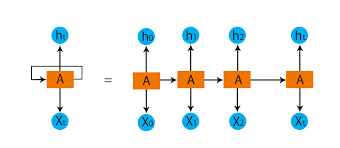
\includegraphics[width=\textwidth]{transformer_images/rnn_image.png}
		\caption{RNN}
		\label{fig:RNN}
	\end{minipage}
	\hfill
	
\end{figure}








\subsubsection{ساختار و عملکرد \lr{RNN}}
شبکه‌های \lr{RNN} دارای حلقهٔ بازگشتی هستند که به مدل این امکان را می‌دهد اطلاعات را در توالی نگه دارد و در هر گام زمانی، ورودی فعلی \( x_t \) و وضعیت قبلی \( h_{t-1} \) را به‌عنوان ورودی دریافت کند
\cite{goodfellow2016deep}:

\begin{equation}
	h_t = \sigma \big( W \cdot x_t + U \cdot h_{t-1} + b \big)
\end{equation}

در اینجا:
\begin{itemize}
	\item \( h_t \) وضعیت مخفی یا حالت در گام زمانی \( t \) است.
	\item \( W \) وزن‌هایی است که به ورودی \( x_t \) اعمال می‌شود.
	\item \( U \) وزن‌های اعمال‌شده به وضعیت قبلی \( h_{t-1} \) است.
	\item \( b \) بایاس مدل است.
	\item \( \sigma \) تابع فعال‌سازی، معمولاً تانژانت هیپربولیک یا سیگموید.
\end{itemize}

با استفاده از این فرایند، مدل این توانایی را دارد که اطلاعات گذشته را در خود ذخیره کرده و در پردازش‌های بعدی از آن‌ها بهره ببرد.

\subsection{مزایا و معایب \lr{RNN}}
در این قسمت به مزایا و معایب شبکه‌های \lr{RNN} می‌پردازیم.

\subsubsection{مزایا:}
\begin{itemize}
	\item \textbf{حفظ وابستگی زمانی:}  
	\lr{RNN} قادر به پردازش توالی‌های طولانی است و می‌تواند اطلاعات را در طول توالی به خاطر بسپارد
	\cite{elman1990finding}.
	
	\item \textbf{کاربردهای گسترده در داده‌های ترتیبی:}  
	این مدل در تحلیل زبان طبیعی، پیش‌بینی سری‌های زمانی و پردازش صوت بسیار موفق عمل می‌کند
	\cite{gers1999learning}.
\end{itemize}

\subsubsection{معایب:}
\begin{itemize}
	\item \textbf{مشکل ناپدید شدن و انفجار گرادیان (\lr{Vanishing and Exploding Gradient}):}  
	در فرایند آموزش با روش پس‌انتشار، اگر توالی داده‌ها طولانی باشد، گرادیان‌ها ممکن است بسیار کوچک یا بزرگ شوند که منجر به ناپایداری در آموزش و کاهش دقت می‌شود
	\cite{hochreiter1998vanishing}.
	
	\item \textbf{محدودیت در پردازش توالی‌های بسیار بلند:}  
	\lr{RNN} در حفظ اطلاعات طولانی‌مدت با مشکل مواجه است و برای پردازش وابستگی‌های طولانی، عملکرد ضعیفی دارد
	\cite{hochreiter1997long,goodfellow2016deep}.
\end{itemize}

\subsection{شبکه‌های حافظه بلندمدت-کوتاه‌مدت (\lr{LSTM})}

\subsubsection{علل پیدایش \lr{LSTM}}
شبکه‌های \lr{LSTM} به عنوان یک راه‌حل برای یکی از بزرگ‌ترین مشکلات شبکه‌های عصبی بازگشتی (\lr{RNN}) معرفی شدند
\cite{hochreiter1997long}.
یکی از برجسته‌ترین مشکلات موجود در \lr{RNN}ها، معضل ناپدید شدن گرادیان (\lr{Vanishing Gradient}) بود که مانع یادگیری وابستگی‌های بلندمدت می‌شد
\cite{hochreiter1998vanishing,goodfellow2016deep}.
برای درک عمیق‌تر این مسأله، ابتدا به توضیح مشکل ناپدید شدن گرادیان و سپس راهکار \lr{LSTM} می‌پردازیم.

\subsubsection{\lr{Gradient Vanishing}}
شبکه‌های \lr{RNN} برای پردازش داده‌های ترتیبی از حلقه‌های بازگشتی بهره می‌برند. در فرایند آموزش \lr{RNN}، از الگوریتم پس‌انتشار خطا از طریق زمان (\lr{Backpropagation Through Time, BPTT}) استفاده می‌شود که گرادیان‌ها را جهت به‌روزرسانی وزن‌ها محاسبه می‌کند
\cite{rumelhart1986learning}.
با این حال، \lr{RNN}ها در یادگیری وابستگی‌های بلندمدت معمولاً ناکام می‌مانند. علت اصلی این امر شامل موارد زیر است:

\begin{itemize}
	\item \textbf{ضریب‌های بازگشتی کوچک‌تر از ۱:}
	در فرایند محاسبهٔ گرادیان‌ها، اگر مقدار مشتقات یا ضرایب در هر مرحله کوچک‌تر از ۱ باشد، ضرب مکرر این ضرایب در طول توالی منجر به کوچک‌شدن گرادیان‌ها به سمت صفر می‌شود؛ پدیده‌ای که به ناپدید شدن گرادیان معروف است
	\cite{hochreiter1998vanishing}.
\end{itemize}

فرمول کلی گرادیان در زمان \( t \) به‌صورت زیر است:

\[
\frac{\partial L}{\partial W} = \prod_{k=1}^{t} \frac{\partial h_k}{\partial h_{k-1}} \cdot \frac{\partial h_t}{\partial L},
\]
در این فرمول، \( \frac{\partial h_k}{\partial h_{k-1}} \) ممکن است مقداری کوچک‌تر از ۱ باشد، و ضرب مکرر آن در طول توالی باعث کاهش شدید مقدار گرادیان می‌گردد.

\begin{itemize}
	\item \textbf{تأثیر مستقیم بر وزن‌ها:}
	زمانی که گرادیان‌ها به صفر نزدیک می‌شوند، وزن‌های مدل عملاً به‌روزرسانی نمی‌شوند و این امر مانع از یادگیری وابستگی‌های طولانی‌مدت در داده‌ها می‌شود
	\cite{goodfellow2016deep}.
\end{itemize}

\subsection{ظهور \lr{LSTM}}
در سال ۱۹۹۷، \lr{Sepp Hochreiter} و \lr{J{\"u}rgen Schmidhuber} شبکه‌های حافظهٔ بلندمدت-کوتاه‌مدت (\lr{LSTM}) را معرفی کردند
\cite{hochreiter1997long}.
انگیزهٔ اصلی توسعهٔ \lr{LSTM} حل مشکل ناپدید شدن گرادیان در شبکه‌های \lr{RNN} بود. این مشکل در مسائل یادگیری داده‌های ترتیبی طولانی مانع می‌شد \lr{RNN} وابستگی‌های بلندمدت را به‌درستی فراگیرد.

\subsubsection{راه‌حل \lr{LSTM} برای پایداری جریان گرادیان‌ها}
\lr{LSTM} با معرفی معماری جدید در شبکه‌های بازگشتی، جریان گرادیان‌ها را در طول توالی پایدار نگه می‌دارد. این کار از طریق اضافه کردن وضعیت سلولی (\lr{Cell State}) و دروازه‌ها (\lr{Gates}) به ساختار \lr{RNN} انجام می‌شود
\cite{gers1999learning}.
این اجزا به \lr{LSTM} امکان می‌دهند:

\begin{enumerate}
	\item اطلاعات غیرضروری را فراموش کند،
	\item اطلاعات مهم جدید را اضافه کند،
	\item اطلاعات مهم قبلی را حفظ کند.
\end{enumerate}

\section{اختار \lr{LSTM}: نوآوری در مقایسه با \lr{RNN}}
\lr{LSTM} شامل اجزای جدیدی است که به آن امکان مدیریت بهتر اطلاعات را می‌دهد:




\subsection{وضعیت سلولی (\lr{Cell State})}
مسیر اصلی ذخیرهٔ اطلاعات در \lr{LSTM} است که می‌تواند اطلاعات مهم را در طول توالی حفظ کند. برخلاف \lr{RNN} که عمدتاً بر خروجی‌های بازگشتی \( h_t \) متکی است، \lr{LSTM} یک مسیر جداگانه برای عبور اطلاعات از وضعیت سلولی دارد که به حفظ گرادیان‌ها کمک شایانی می‌کند
\cite{hochreiter1997long}.


 \begin{figure}[h]
	\centering
	\begin{minipage}[b]{0.7\textwidth}
		\centering
		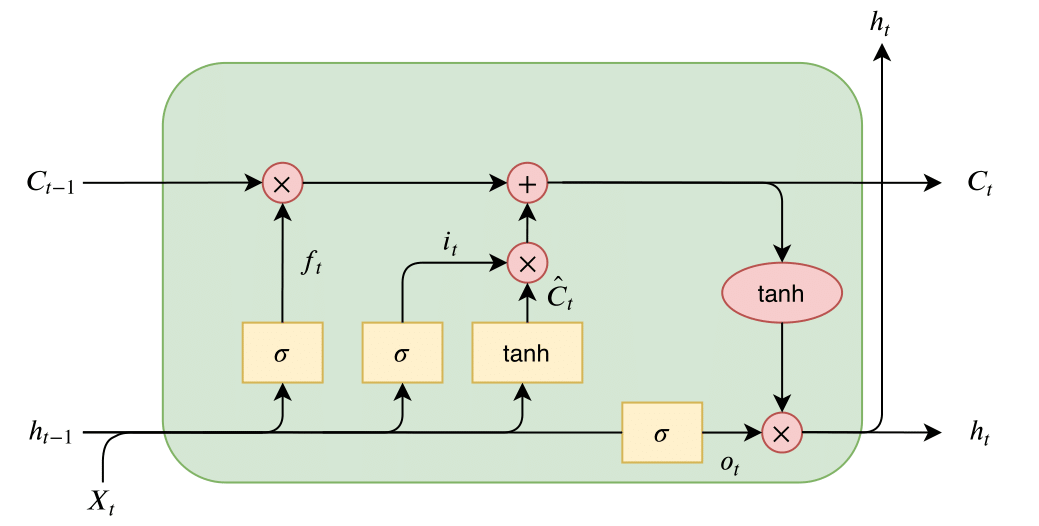
\includegraphics[width=\textwidth]{transformer_images/lstm.png}
		\caption{LSTM}
		\label{fig:LSTM}
	\end{minipage}
	\hfill
	
\end{figure}


\subsection{دروازه‌ها (\lr{Gates})}
دروازه‌ها نقش فیلترهای اطلاعاتی را دارند که جریان اطلاعات را در طول فرایند یادگیری کنترل می‌کنند:

\begin{itemize}
	\item \textbf{دروازهٔ فراموشی (\lr{Forget Gate}):}
	تعیین می‌کند چه اطلاعاتی از وضعیت سلولی باید حذف شود
	\cite{gers1999learning}:
	\[
	f_t = \sigma \big( W_f \cdot [h_{t-1}, x_t] + b_f \big),
	\]
	\[
	f_t:\text{ میزان فراموشی برای هر عنصر از وضعیت سلولی},
	\]
	\[
	\sigma:\text{ تابع سیگموید (خروجی بین ۰ و ۱)}.
	\]
	در صورت \( f_t = 0 \)، اطلاعات حذف می‌شود و در صورت \( f_t = 1 \)، حفظ می‌شود.
	
	\item \textbf{دروازهٔ ورودی (\lr{Input Gate}):}
	تعیین می‌کند چه اطلاعات جدیدی باید به وضعیت سلولی اضافه شود:
	\[
	i_t = \sigma \big( W_i \cdot [h_{t-1}, x_t] + b_i \big),
	\]
	\[
	\tilde{C}_t = \tanh \big( W_C \cdot [h_{t-1}, x_t] + b_C \big),
	\]
	که در آن \( i_t \) میزان اطلاعات جدید و \( \tilde{C}_t \) مقدار جدید قابل اضافه‌شدن به وضعیت سلولی را نشان می‌دهد.
	
	\item \textbf{دروازهٔ خروجی (\lr{Output Gate}):}
	تعیین می‌کند چه اطلاعاتی از وضعیت سلولی به خروجی منتقل شود:
	\[
	o_t = \sigma \big( W_o \cdot [h_{t-1}, x_t] + b_o \big),
	\]
	\[
	h_t = o_t \cdot \tanh(C_t).
	\]
\end{itemize}

\subsection{به‌روزرسانی وضعیت سلولی}
وضعیت سلولی \( C_t \) با استفاده از اطلاعات جدید و قدیمی به‌روزرسانی می‌شود:
\[
C_t = f_t \cdot C_{t-1} + i_t \cdot \tilde{C}_t.
\]
این ساختار باعث می‌شود اطلاعات قدیمی مهم حفظ و داده‌های غیرضروری حذف شوند.

\subsubsection{علت پایداری گرادیان در \lr{LSTM}}
\begin{itemize}
	\item \textbf{حذف ضرب‌های مکرر:}
	برخلاف \lr{RNN} که به ضرب‌های مکرر وزن‌ها و گرادیان‌ها وابسته است، \lr{LSTM} با مسیر جداگانهٔ وضعیت سلولی، از کاهش نمایی گرادیان جلوگیری می‌کند
	\cite{hochreiter1998vanishing}.
	
	\item \textbf{استفاده از توابع سیگموید و تانژانت هیپربولیک:}
	توابع سیگموید در دروازه‌ها و تانژانت هیپربولیک در وضعیت سلولی مقادیر را محدود می‌کنند و مانع از انفجار گرادیان می‌شوند
	\cite{gers1999learning,goodfellow2016deep}.
	
	\item \textbf{مدیریت اطلاعات توسط دروازه‌ها:}
	دروازه‌های فراموشی و ورودی به مدل اجازه می‌دهند تنها اطلاعات مهم حفظ شود و داده‌های غیرضروری حذف شوند؛ این موضوع از پیچیدگی محاسباتی غیرضروری جلوگیری می‌کند
	\cite{hochreiter1997long}.
\end{itemize}


%\subsection{مقایسه RNN  و LStm:}


\begin{table}[h!]
	\centering
	\resizebox{\columnwidth}{!}{%
		\begin{tabular}{|c|c|c|}
			\hline
			\textbf{ویژگی} & \textbf{RNN} & \textbf{LSTM} \\ \hline
			\textbf{مشکل ناپدید شدن گرادیان} & وجود دارد & برطرف شده \\ \hline
			\textbf{توانایی حفظ وابستگی‌های طولانی‌مدت} & محدود به وابستگی کوتاه‌مدت & بسیار خوب \\ \hline
			\textbf{ساختار دروازه‌ها} & ندارد & دارای دروازه‌های فراموشی، ورودی و خروجی \\ \hline
			\textbf{پایداری گرادیان} & ضعیف & پایدار \\ \hline
		\end{tabular}%
	}
	\caption{مقایسه ویژگی‌های RNN و LSTM}
\end{table}



\subsection{مشکلات کلی \lr{RNN} و \lr{LSTM} و ظهور ترنسفورمرها}
شبکه‌های بازگشتی \lr{RNN} و \lr{LSTM} توانستند بسیاری از مشکلات و محدودیت‌های مدل‌های اولیه را حل کنند؛
اما همچنان با چالش‌ها و محدودیت‌هایی مواجه بودند که در مسائل پیچیده‌تر، مانند ترجمهٔ زبان یا تحلیل داده‌های بلندمدت و حجیم، مشکلات جدی ایجاد می‌کردند
\cite{hochreiter1997long,goodfellow2016deep}.
این مشکلات در نهایت به پیدایش ترنسفورمرها (\lr{Transformers}) منجر شد
\cite{vaswani2017attention}.
در ادامه، مهم‌ترین محدودیت‌های \lr{RNN} و \lr{LSTM} مورد بررسی قرار می‌گیرند.

\subsubsection{مشکل وابستگی ترتیبی در \lr{RNN}ها و \lr{LSTM}ها}
\lr{RNN}ها و \lr{LSTM}ها داده‌ها را به‌صورت ترتیبی پردازش می‌کنند؛ به این معنی که برای پردازش داده‌های گام زمانی \( t \)، باید تمامی داده‌های قبلی (\( t-1 \)) پردازش شده باشند
\cite{rumelhart1986learning,hochreiter1997long}.
این ویژگی مشکلات زیر را ایجاد می‌کند:
\begin{itemize}
	\item \textbf{غیرقابل موازی‌سازی:}  
	به دلیل وابستگی ترتیبی، پردازش داده‌ها به‌صورت موازی ممکن نیست و همین امر باعث افزایش زمان محاسباتی می‌شود. در داده‌های بلند (مانند متن‌های طولانی یا سری‌های زمانی بزرگ)، این مشکل نمود بیشتری دارد.
	
	\item \textbf{کندی آموزش و استنتاج:}  
	پردازش خطی داده‌ها موجب می‌شود زمان آموزش و پیش‌بینی مدل‌ها به‌شدت افزایش یابد، به‌ویژه زمانی که با حجم زیادی از داده مواجه هستیم.
\end{itemize}

\subsubsection{محدودیت در یادگیری وابستگی‌های بسیار طولانی}
با وجود پیشرفت \lr{LSTM} در یادگیری وابستگی‌های بلندمدت نسبت به \lr{RNN}های معمولی، این مدل‌ها همچنان در یادگیری وابستگی‌های بسیار بلند، مانند ارتباط بین کلمات در جملات دور از هم یا درک ساختار کلی یک متن، محدودیت دارند
\cite{hochreiter1998vanishing}:
\begin{itemize}
	\item \textbf{مشکل در داده‌های بسیار طولانی:}  
	حتی در \lr{LSTM} نیز ظرفیت حفظ اطلاعات محدود است و با افزایش طول توالی، دقت مدل افت می‌کند.
	
	\item \textbf{تأثیر تدریجی داده‌های اولیه:}  
	داده‌های ابتدایی توالی ممکن است با گذشت زمان اهمیت خود را از دست بدهند، چراکه گرادیان‌ها به‌تدریج ضعیف‌تر می‌شوند.
\end{itemize}

\subsubsection{پیچیدگی محاسباتی و حافظه}
\lr{LSTM}ها به علت ساختار پیچیده‌ای که شامل چندین ماتریس ضرب (برای دروازه‌های فراموشی، ورودی و خروجی) و به‌روزرسانی وضعیت سلول است، به حافظه و محاسبات زیادی نیاز دارند
\cite{goodfellow2016deep}:
\begin{itemize}
	\item \textbf{نیاز به حافظه بیشتر:}  
	برای ذخیرهٔ وضعیت سلولی و گرادیان‌ها، \lr{LSTM}ها به حافظهٔ بیشتری نسبت به مدل‌های ساده‌تر احتیاج دارند.
	
	\item \textbf{هزینهٔ محاسباتی بالا:}  
	در داده‌های حجیم، انجام محاسبات سنگین می‌تواند اجرای مدل را بسیار کند سازد.
\end{itemize}

\subsubsection{مشکل پردازش وابستگی‌های غیرمتوالی}
\lr{RNN}ها و \lr{LSTM}ها به‌طور طبیعی برای یادگیری وابستگی‌های محلی و متوالی مناسب هستند. اما در مسائلی مانند ترجمهٔ زبان یا تحلیل متون، روابط غیرمحلی و غیرمتوالی نیز اهمیت دارند
\cite{bahdanau2014neural}.
به‌عنوان مثال، در جمله‌ای طولانی ممکن است کلمه‌ای در ابتدای جمله با کلمه‌ای در انتهای جمله ارتباط معنایی داشته باشد. \lr{RNN}ها و \lr{LSTM}ها برای یادگیری این‌گونه وابستگی‌ها محدودیت دارند.

\subsubsection{گرادیان‌های ناپایدار و مشکلات بهینه‌سازی}
با وجود بهبودهایی که \lr{LSTM} نسبت به \lr{RNN} در پایداری گرادیان ارائه داد، هنوز هم:
\begin{itemize}
	\item \textbf{مسائل گرادیان‌های ناپایدار:}  
	در توالی‌های بسیار بلند، گرادیان‌ها ممکن است همچنان دچار کاهش یا حتی در مواردی انفجار شوند.
	
	\item \textbf{مشکلات بهینه‌سازی:}  
	در مسائلی با ساختار پیچیده، یافتن مینیمم مناسب تابع هزینه برای \lr{RNN}ها و \lr{LSTM}ها دشوار است.
\end{itemize}

\subsubsection{نیاز به مدلی با ظرفیت بیشتر و سرعت بالاتر}
\begin{itemize}
	\item \textbf{مدل‌های بزرگ‌تر:}  
	برای مسائل پیچیده‌تر، به مدل‌هایی با تعداد پارامتر بالاتر نیاز است؛ اما \lr{RNN}ها و \lr{LSTM}ها به‌دلیل محدودیت در حافظه و پردازش، پاسخ‌گوی این نیاز نیستند.
	
	\item \textbf{کارایی در داده‌های چندوجهی (\lr{Multimodal}):}  
	برای داده‌هایی که ترکیبی از اطلاعات متنی، صوتی و تصویری هستند، \lr{RNN}ها و \lr{LSTM}ها توانایی لازم جهت پردازش موازی این اطلاعات را ندارند.
\end{itemize}

در مجموع، وابستگی ترتیبی در \lr{RNN} و \lr{LSTM} مانعی اساسی برای استفاده از این مدل‌ها در مسائل پیچیده و بزرگ بود که درنهایت به ظهور ترنسفورمرها منتهی شد
\cite{vaswani2017attention}.
ترنسفورمرها با طراحی مبتنی بر موازی‌سازی و مکانیزم توجه (\lr{Attention Mechanism})، این محدودیت را برطرف کرده و راه‌حلی کارآمدتر برای پردازش داده‌های ترتیبی ارائه دادند.



